\documentclass[journal]{IEEEtran}
\usepackage{blindtext}
\usepackage{graphicx}
\usepackage{url}

\begin{document}
\title{Click-Through Rate Prediction for Sponsored Search Advertising in Microsofts Bing Search Engine}
\author{Craig Heptinstall Crh13- 110005643 \\
SEM6120\\Institute of Computer Science\\Aberystywth University}

\maketitle


\begin{abstract}
In 2009, a paper by Thor Graepel \cite{bing-paper} described a winning click-through rate (CTR) prediction algorithm used for sponsored search in Microsoft's Bing search engine (the authors named this adPredictor). The paper introduced a Bayesian online learning concept that was chosen to replace the previous CTR algorithm. Here this paper looks at the concepts used in the adPredictor algorithm and how appropriate certain aspects of the task were identified and dealt with. Following an evaluation of the algorithm and paper itself, there are of course, always further improvements possible to any algorithm. Using other research, suggestions have been presented to increase the efficiency of the solution, especially over the web (since this algorithm should work efficiently during real time searches).

\end{abstract}

\section{Sponsored search}
Sponsored search is considered as one of the most profitable business models today, and according to several sources of analytic services such as analytics-magazine \cite{business-model} the four top search engines(Bing, Google, Yahoo and Baidu) make in excel of \$37 billion. Bing however gets the lion share with over \$25 billion of the total coming its own way. Therefore, keeping this amount on an upward trend requires appropriate and efficient advertisements. \\
Sponsored search uses two key aspects to the use of a search engine that can be applied to providing advertisements:
\begin{itemize}
\item The query the users enter- This indicates the requirement of the user
\item Users clicking on advertisements- This gives users the opportunity to see advertiser's pages
\end{itemize}
In order to get the advertisements that is useful to the search engine (in terms of revenue), the advertisers (in terms of clicks on their links), and user's needs (In terms of relevant adverts), CTR prediction is a most vital part of a search engine.

\subsection{Click rate prediction}
The paper begins by detailing what click rate prediction is and how it fits into the web framework that is the Bing search engine. Getting an accurate metric for where advertisements will be clicked is important to the user, and more so the search engine. By being able to get the probability of an advert being clicked, the authors are able to increase further the possible profitability of the search engine via advert placement, and assisting the choice of adverts to be displayed. \\
Although the paper describes CTR well as a starting point, the graph in figure \ref{fig:CTR} shows an example of how keywords and where they are placed on a page affect the CTR. By having a good predictor, the keywords and placement of adverts will be more informed before they are added to search.

\begin{figure}[!ht]
  \caption{CTR based on position of advertisement. Image taken from a marketing explanation of CTR \cite{ctr-image}.}
  \centering
  \label{fig:CTR}
    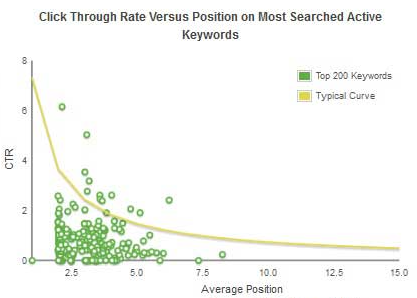
\includegraphics[width=0.5\textwidth]{CTR}
\end{figure}

\subsection{Keywords auction}
In order to grasp the whole concept of CTR prediction, keyword auction is something that the paper describes as an important feature in displaying advertisements in their specific places. Rather than having selected ads chosen by the selecting algorithm just place them in any order on the screen, keyword auction uses an algorithm known as generalized second price (GSP). This ensures that advertisers pay appropriate amounts referring to what position they appear on a search page. \\
GSP is a fairly simple algorithm \cite{keyword-auction}, which takes in a number of bids from bidders (in this case advertisers) all of which specify amounts they are willing to pay for clicks on adverts related to certain keywords. Following the auction, the bids with the highest prices win the best place, but only pay the second highest bid price. After this, the second highest pays the second highest bid and so on. Predicting which advertisements will be used by users heavily relies on the results from a GSP, which the adPredictor paper expands on with constraints that this way of generating advertisements brings.

\section{Challenges approached by adPredictor}
There were a number of existing problems that needed to be solved by any CTR predictor in order to create an efficient solution that would be enough to replace Bing’s previous predictor. These range from getting suitable input features for the predictor, to evaluating the performance of the predictor itself. This section of the paper looks at each of these in relation to what the adPredictor authors had to accomplish in order for their solution to work.

\subsection{Features and impressions}
With any machine learning algorithm, there must be appropriate input features that can represent variables used to produce outcomes (in this case binary). Because the web is quite diverse, and is forever changing, many different aspects of a user’s actions should be considered when predicting click through rates. The authors of adPredictor questions the availability of inputs, and comes to a conclusion that at least three main categories should be considered when attempting to create the probability of a user’s click:
\begin{enumerate}
\item Ad features- The adverts themselves, including links, text on the adverts and the campaign of the ad.
\item Query features- These are directly entered by the user, such as words searched by the user.
\item Context features- Indirectly given by the user, to personalise adverts more. These could be the location of the user, time and date to name a few.
\end{enumerate}
Because of the vast size features possible, the complexity of the algorithm had to be considered, alongside the speed of which the predictor would function. Selecting good features is one of the building blocks of any machine learning algorithm. In a lecture by Jeff Howbert at Washington University \cite{washington}, he mentions the ‘Curse of dimensionality’ and states that as features increase the volume of feature space increases too. This makes data harder to understand and results in an increase of difficulty of achieving statistical significances.

\subsection{Isolated predictions}
The next task challenging the authors was the testing of the predictor. In order to actually see results from their algorithm, there was the task of seeing how well it performed. Although the author suggests a number of ways that machine learning predictors can be tested (AUC (area under the receiver operator curve), or log-likelihood of test data), with the predictor being part of a larger system means that different goals from users, advertisers and the search engine may conflict resulting in inaccurate test results.

\subsection{Web implementations}
Dynamic web
Computational cost

\section{Results and analysis}

\section{Alternative proposed solution}

\subsection{Results and comparisons}

\section{Conclusion}

\appendices

\ifCLASSOPTIONcaptionsoff
  \newpage
\fi

\begin{thebibliography}{1}

\bibitem{bing-paper}
T.~Graepel, \emph{Web-Scale Bayesian Click-Through Rate Prediction for Sponsored Search Advertising in Microsoft's Bing Search Engine}, \hskip 1em plus
  0.5em minus 0.4em\relax Microsoft Research Ltd, 2010.
  
\bibitem{business-model}
P.~Quinn, \emph{Sponsored search advertising}, \hskip 1em plus
  0.5em minus 0.4em\relax Analytics Magazine, \emph{\url{http://www.analytics-magazine.org/may-june-2012/580-online-analytics-sponsored-search-advertising}}, 2012.
  
\bibitem{keyword-auction}
B.~Edelman, \emph{Internet Advertising and the Generalized Second-Price Auction:
Selling Billions of Dollars Worth of Keywords}, \hskip 1em plus
  0.5em minus 0.4em\relax \url{www.benedelman.org}, 2006.
  
\bibitem{ctr-image}
L.~Kim, \emph{Five Must-Have Insights for Better PPC Campaign Performance}, \hskip 1em plus
  0.5em minus 0.4em\relax Marketing Profs, \emph{\url{http://www.marketingprofs.com/articles/2014/24562/five-must-have-insights-for-better-ppc-campaign-performance}}, 2014.
  
\bibitem{washington}
J.~Howbert, \emph{Machine Learning: Feature Creation and Selection
}, \hskip 1em plus
  0.5em minus 0.4em\relax \url{http://courses.washington.edu}, 2012.
  
\end{thebibliography}

\end{document}


